\section{Front-end and SiPM results}\label{sec:results}
A complete readout slice consisting of a KDB with 4 Hamamatsu S10362-11-050P SiPMs, 4 SensL MicroFC-10035-SMT-GP SiPMs, a 4m cable, a FEB64 front-end card, a DAQ interface module and a DAQ PC running the DATE environment has been tested.
Signals generated by dark counts events have been used to produce their Single Photon Spectrum (SPS). The different intensities in the generated signals correspond to different number of fired pixel in the sensors during the electronic sample time (1~$\mu s$). As observed in the most left peak in both plots in figure~\ref{fig:dk}, the SPS indicates good photon counting capability for both sensors, allowing to identify different peaks which are used to produce the absolute calibration of the channels, in number of ADC Counts per single photoelectron. The main difference between them is the dark count rate (see table~\ref{table:SiPMpro}).

\begin{figure}[h!]
  \centering
  \subfloat[\textit{Hamamatsu S10362-11-050P}]{%\label{fig:cabling:}
  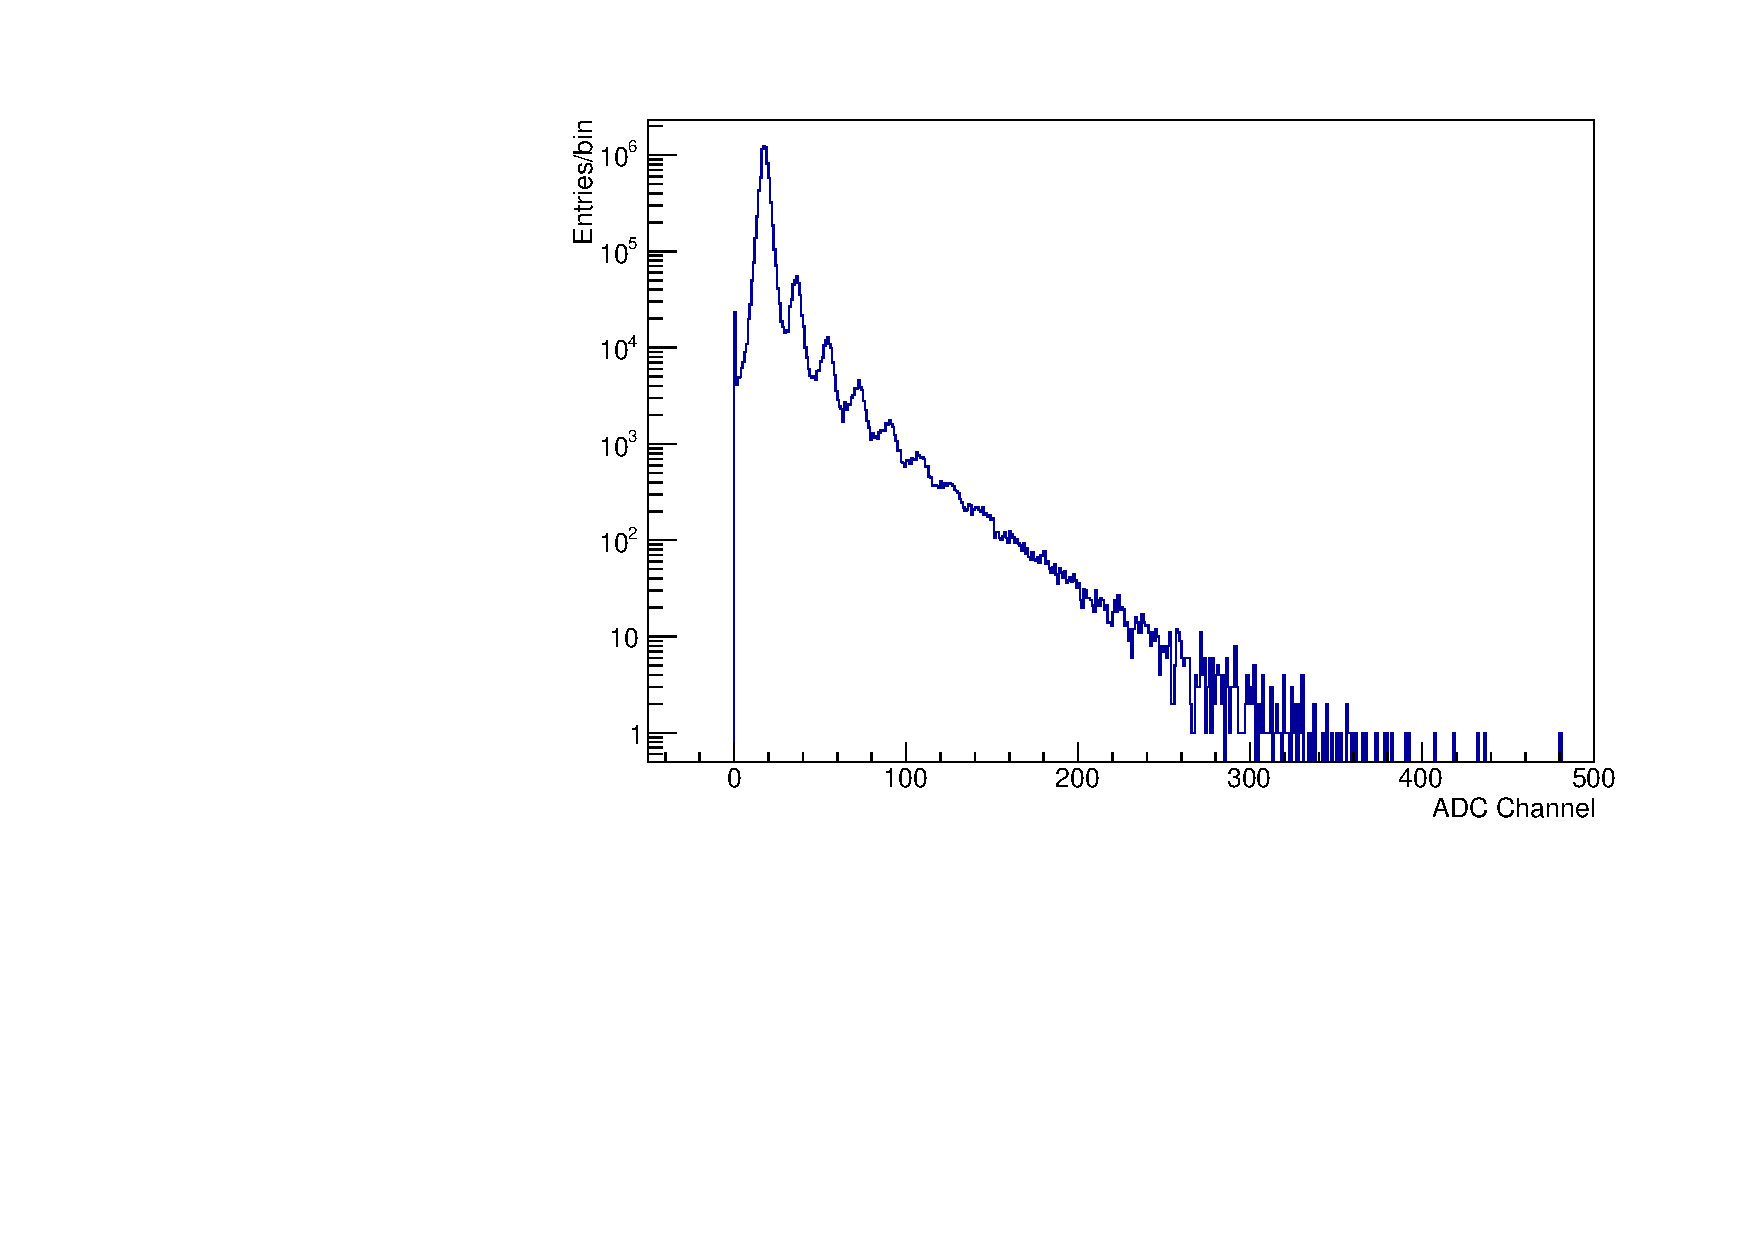
\includegraphics[height=0.3\textwidth]{SpecHama.pdf}}   
  \hspace{5mm}             
  \subfloat[\textit{SensL MicroFC-10035-SMT-GP}]{%\label{fig:ad:ads7883}
  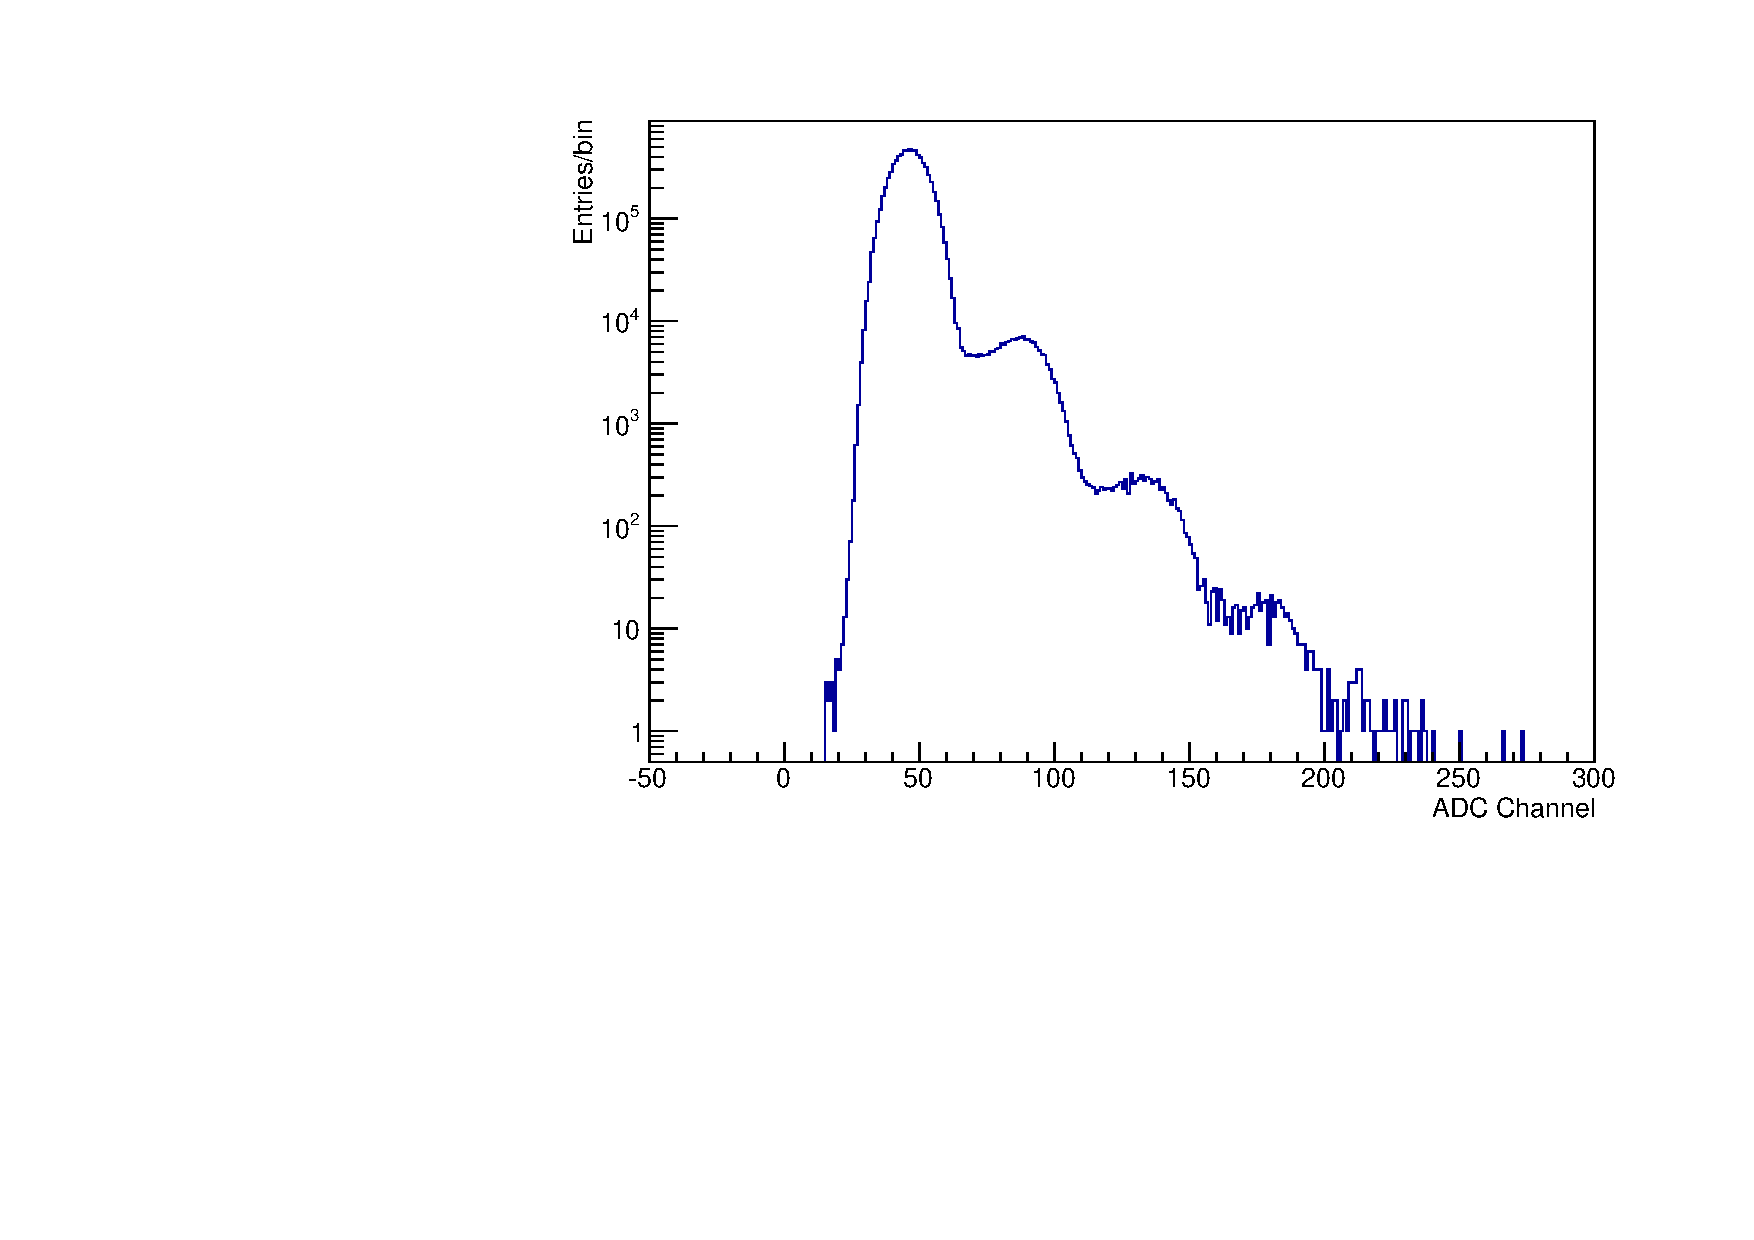
\includegraphics[height=0.3\textwidth]{SpecSensL.pdf}}
  \caption{\textit{Single photon spectrum for dark current events}}
  \label{fig:dk}
\end{figure}

As Hamamatsu and SensL SiPM have different gain at their operating voltage, the gain in the analog stage of the front-end has been adjusted to fit the same dynamic range with both sensors, trying to obtain the same gain at the end of the acquisition chain. From figure~\ref{fig:dk} we can obtain the gain of both photosensors, which are $16.09~ADC counts/V$ for the Hamamatsu S10362-11-050P SiPM, and $17.34~ADC counts/V$ for the SensL MicroFC-10035-SMT-GP.

The dynamic performance of both SiPMs was also tested, obtaining the gain vs temperature and gain vs bias voltage dependence, in the same conditions. As can be seen in figure~\ref{fig:temp}, Hamamatsu SiPMs have $\sim0.4~~ADC counts/\degree$ and SensL SiPMs have $\sim0.2~ADC counts/\degree$. This result indicates that SensL SiPMs are easier to compensate for temperature fluctuations while running.

\begin{figure}[h!]
  \centering
  \subfloat[\textit{Hamamatsu S10362-11-050P}]{%\label{fig:cabling:}
  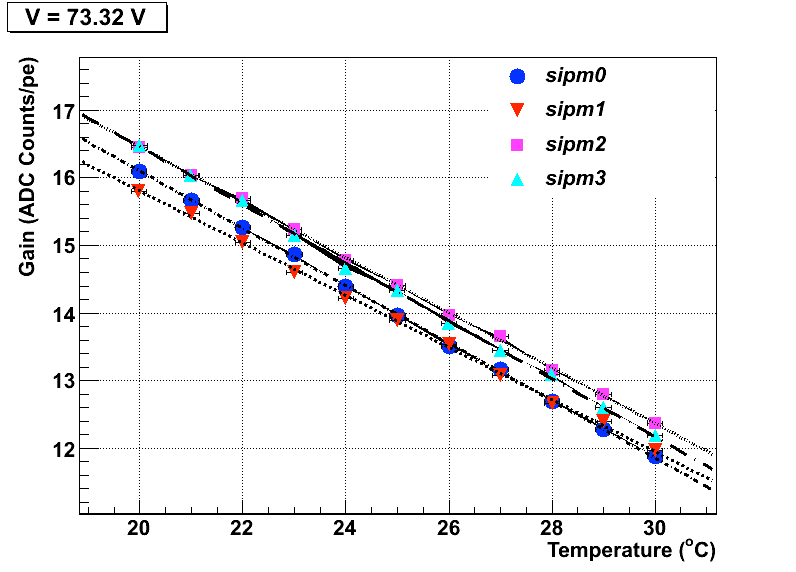
\includegraphics[height=0.3\textwidth]{GvsT.png}}   
  \hspace{5mm}             
  \subfloat[\textit{SensL MicroFC-10035-SMT-GP}]{%\label{fig:ad:ads7883}
  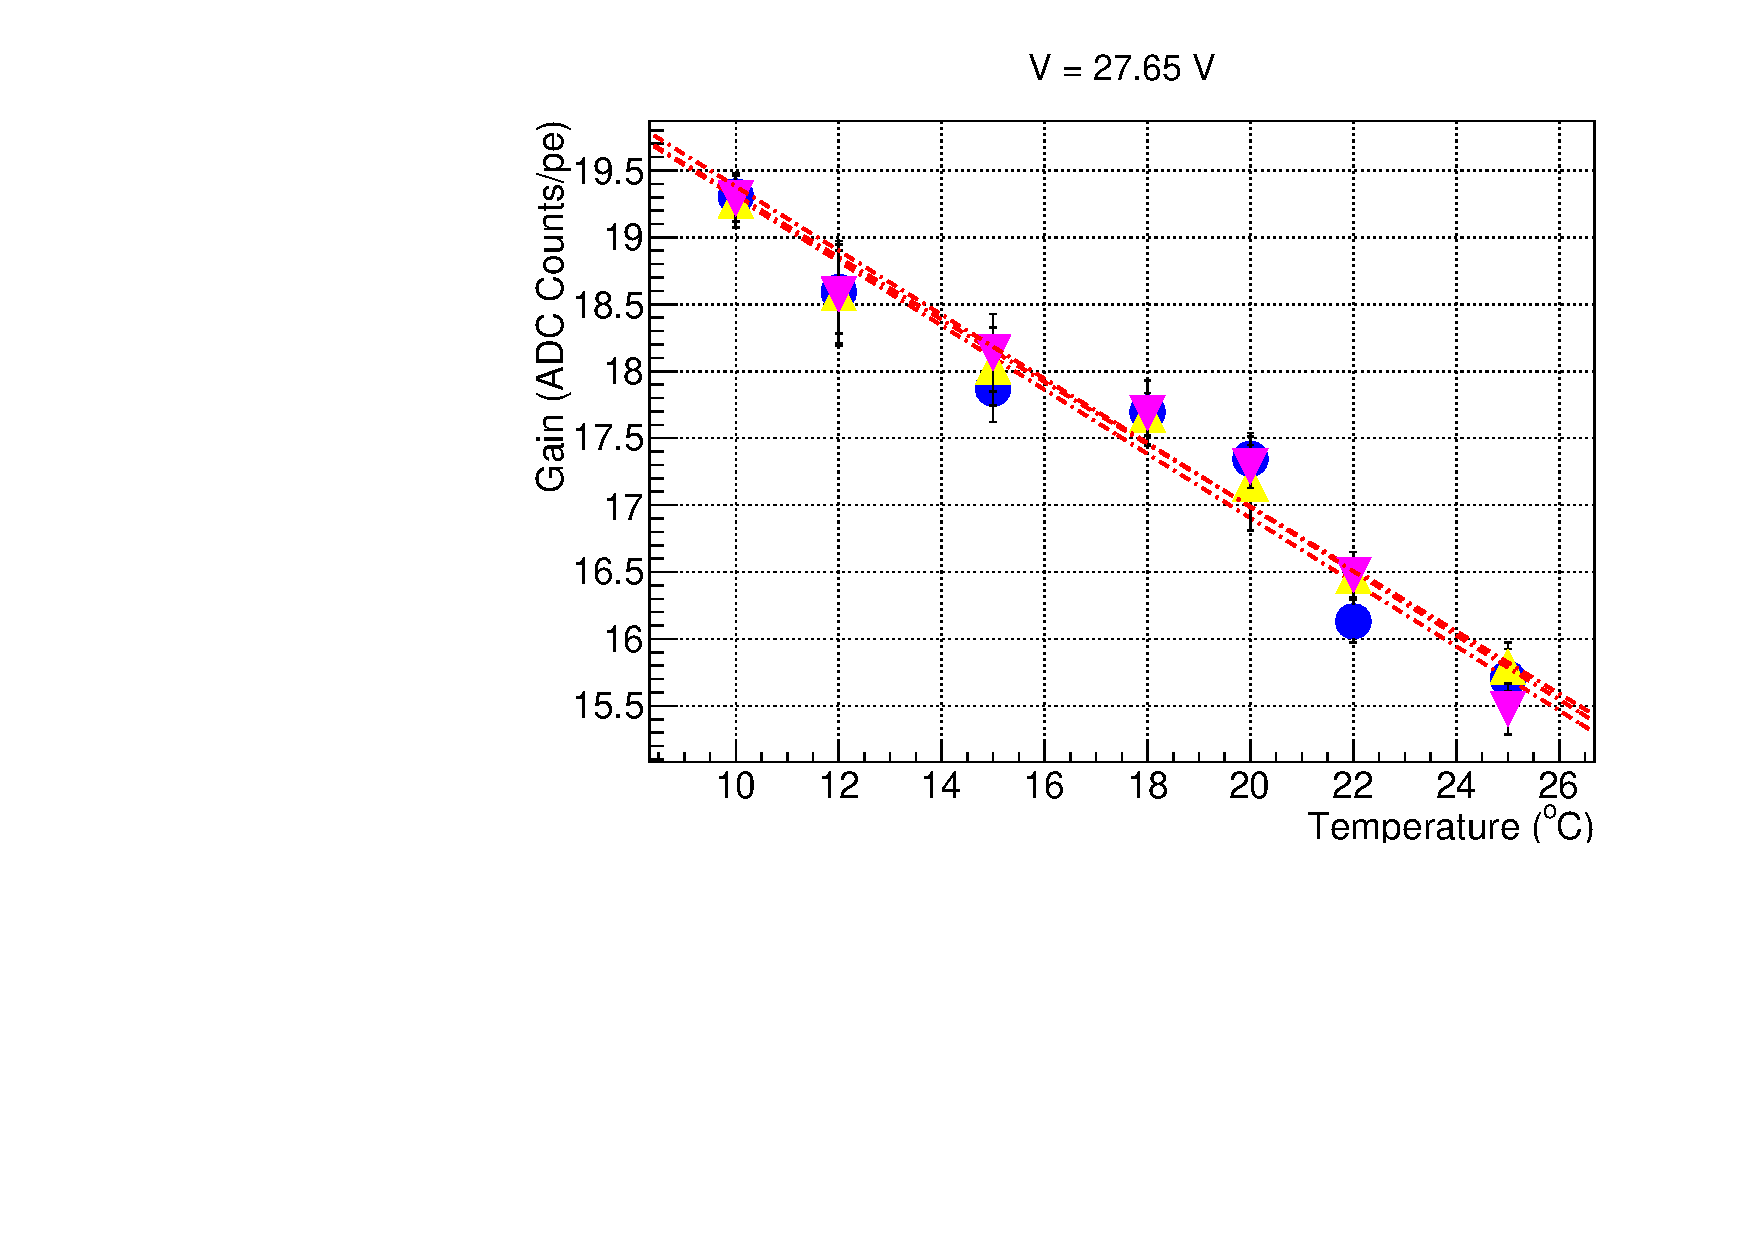
\includegraphics[height=0.3\textwidth]{GvsTsnsl.pdf}}
  \caption{\textit{Gain dependence as a function of temperature}}
  \label{fig:temp}
\end{figure}

At the same time, gain dependence with bias voltage has been analyzed (see figure~\ref{fig:bias}), showing a dependence of $\sim10~ADC counts/V$ in the Hamamatsu SiPMs and $\sim5ADC counts/V$ in the SensL SiPMs. These results showed also an advantage for the SensL sensors, because less gain dependence means lower gain spread in a DICE-Board.

\begin{figure}[h!]
  \centering
  \subfloat[\textit{Hamamatsu S10362-11-050P}]{%\label{fig:cabling:}
  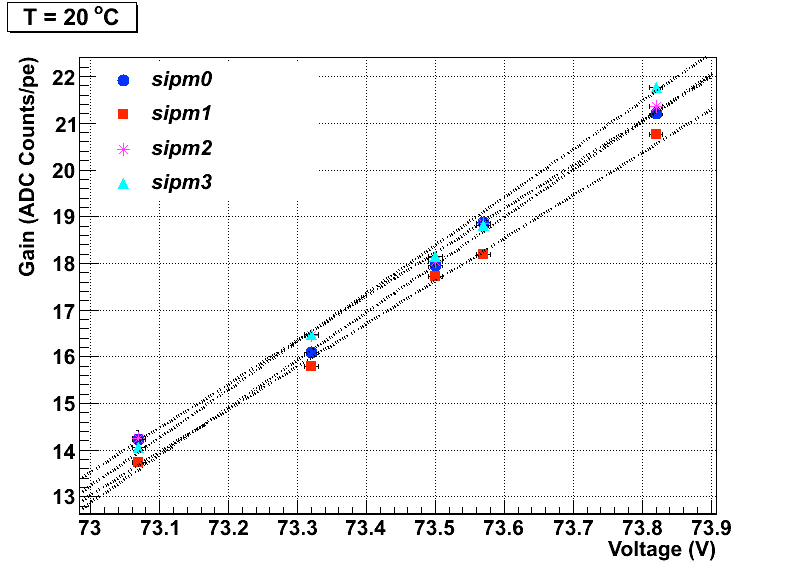
\includegraphics[height=0.3\textwidth]{GvsV.png}}   
  \hspace{5mm}             
  \subfloat[\textit{SensL MicroFC-10035-SMT-GP}]{%\label{fig:ad:ads7883}
  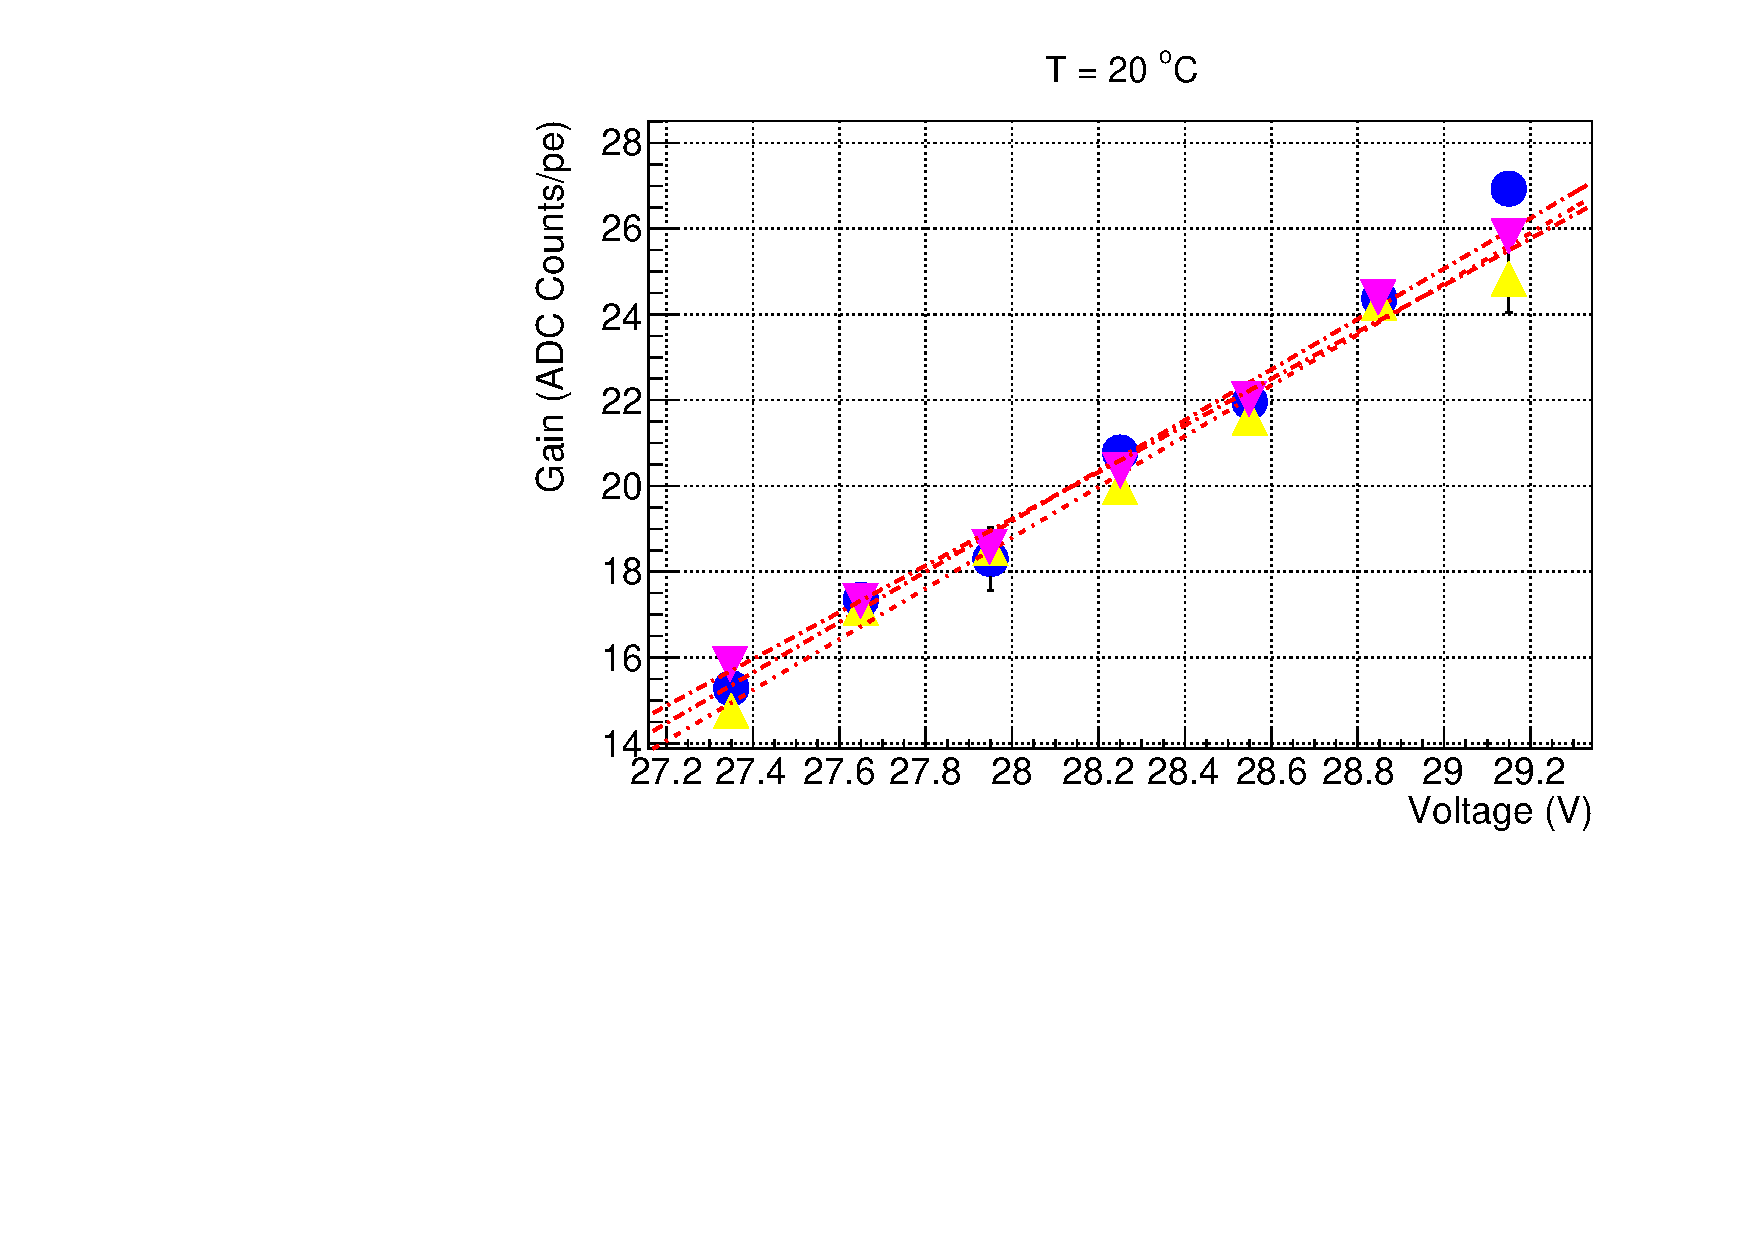
\includegraphics[height=0.3\textwidth]{GvsVsnsl.pdf}}
  \caption{\textit{Gain dependence as a function of bias voltage}}
  \label{fig:bias}
\end{figure}

